%==============================================================================
\section{Experiments}
\label{sec:experiments}
%==============================================================================
% This section presents the case study experiment. First, we describe the environment in which the experiment was carried out and present the scenarios used, the observed variables. Next, we describe the current task scheduling model and the results obtained with this model. In the same way, we describe the proposed model for optimization of the scheduling of tasks and the results obtained. Finally, we compare and discuss the results obtained in each case.
Esta seção apresenta os experimentos realizados para aferição do desempenho do processamento de mensagens no processo de integração com o modelo proposto, que utiliza múltiplos pools com um número de threads ótimo ou próximo de ótimo, obtidos pelo algoritmo baseado no PSO. O experimento compara os resultados obtidos com o modelo proposto e os resultados obtidos com o modelo tradicional que utiliza um único pool e adota a política FIFO para agendamento do processamento das mensagens pela execução das tarefas. 

Primeiro, descrevemos o ambiente em que o experimento foi realizado, apresentamos os cenários utilizados e as variáveis observadas. Em seguida, descrevemos o modelo de tradicional e os resultados obtidos com este modelo. Do mesmo modo, descrevemos o modelo proposto e os resultados obtidos. Finalmente, comparamos e discutimos esses resultados.
%==============================================================================
\subsection{Environments}
\label{subsec:enviroments}
%==============================================================================
Para implementação dos algoritmos e testes primários, foi utilizado computador com sistema operacional Microsoft Windows 10 Education, Intel (R) Core (TM) i5-5200U CPU, 2.20 GHz; 2195 Mhz, 2 núcleos, 4 processadores lógicos, memória RAM de 4.00 GB.

Já para as experimentações computacionais de alto desempenho, com taxa de entrada de mensagens acima de ... e processos de integração acima de ... tarefas, foi utilizado um servidor com a seguinte configuração: armazenamento SAS de 6 Gb, 12 unidades de 2U, dois controladores de cache de 4 GB; seis discos de 2TB, 2.7 K rpm, NLSAS 12Gbps; cache Intel Xeon E5-4610 v4 1.8GHz de 25M, QPI de 6.4 GT / s, sem turbo, HT, dez núcleos / vinte segmentos; três discos SAS 2.5, 12Gbps de 300GB; vinte e quatro pentes de memória RDIMM de 16 GB, 2400 MT / s; RAID5 com três a seis discos; duas fontes de alimentação redundantes.

De modo similar, utilizou-se o software Matlab~\cite{leonard1995}, versão R2013, para criar e testar os programas, os quais foram posteriormente implementados na linguagem Java, versão ...
Para geração de gráficos e tabelas e dados estatísticos, utilizou-se o software Excel, do pacote Microsoft Office 2016.
%==============================================================================
\subsection{Description}
\label{subsec:description}
%==============================================================================
%               - apresentar informações do hardware sobre o qual se executa a experimentação (executaremos no servidor do GCA)
%               - apresentar as variáveis a serem medidas e que permitirão uma posterior comparação. Quais seriam elas?
%                  . número de workunits processadas em um intervalo de tempo? 
%                  . número de mensagens processadas em um intervalo de tempo?
%                  . tempo de inatividade das threads?
%                  ... 
%               - descrever os cenários de experimentação, ou seja, o que iremos variar em cada experimento? 
%                  . taxa de entrada de workunits na fila? 
%                  . número de threads no pool? 
%                  Um cenário é a combinação dessas variáveis, por exemplo: taxa 1 e pool com 4 threads; taxa 2 e pool com 4 threads; ...               
Para obter o tempo total médio de processamento das mensagens (TTAP) e comparar o modelo tradicional com o proposto, foram implementados dois programas. O primeiro simula a execução das tarefas por meio de um único pool de threads e o segundo simula a execução das mesmas tarefas com um pool de threads para cada uma das tarefas, sendo que a soma do número de threads em todos os pools é igual ao numero de threads do pool único do modelo tradicional. Para o modelo proposto, implementamos um algoritmo baseado na metaheurística PSO para encontrar a melhor cofiguração para os pool de threads dedicados a cada tarefa, ou seja, o número de threads que cada pool deve conter, para encontrar a solução ótima ou próxima da ótima, a qual gere o menor tempo total médio de processamento das mensagens. Este algoritmo recebe como parâmetro de entrada o número de soluções que devem ser testadas, que é o critério de parada no nosso algoritmo de otimização. Os demais parâmetros de entrada para os dois programas são:
\begin{enumerate}
                 \item Número total de threads
                 \item Número total de mensagens a serem processadas
                 \item Vetor contendo os tempos de processamentos das tarefas. 
\end{enumerate}
No parâmetro 3, o número de colunas do vetor define o número de tarefas a serem executadas e o índice da coluna define a ordem da execução. 
A Figura~\ref{fig:inputs} mostra a interface para os parâmetros de entrada.
\begin{figure}[h]
\begin{minipage}[c]{0.49\linewidth}
\centering
 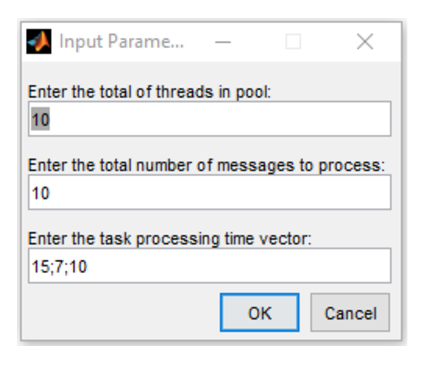
\includegraphics[width=1\linewidth]{./figs/inputs_FIFO.eps}
\end{minipage}
\begin{minipage}[c]{0.49\linewidth}
\centering
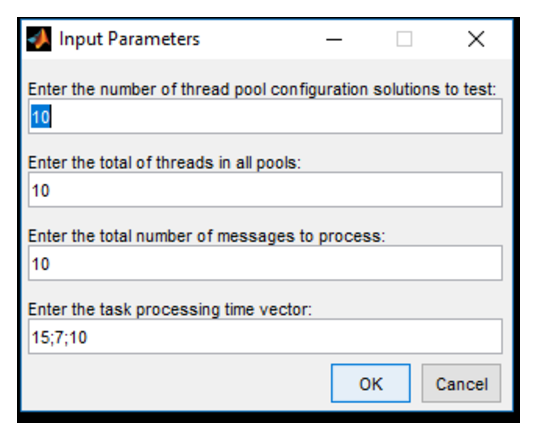
\includegraphics[width=1\linewidth]{./figs/inputs.eps}
\end{minipage}
 \caption{Input interface of the programs.}
\label{fig:inputs}
\end{figure}
Os programas geram uma matriz  com os tempos finais de processamento de cada mensagem por cada uma das tarefas do fluxo. O índice da linha da matriz representa a tarefa executada e o índice da coluna representa a mensagem. O tempo total médio de processamento das mensagens é calculado por meio da média aritmética dos tempos finais das mensagens na última tarefa do fluxo. O programa mostra graficamente a sequência do processamento das mensagens nas tarefas. A Figura~\ref{fig:graphic_sequence} mostra um exemplo dessa sequência. O programa mostra também o tempo total médio de processamento das mensagens, conforme mostrado na Figura~\ref{fig:outputs}. No caso do modelo proposto, mostra a configuração dos pools que resulta no mínimo TTAP. Assim, os parâmetros de saída fornecidos pelo programa são:
\begin{enumerate}
                 \item Matriz de tempos finais de processamento das mensagens.
                 \item Tempo total médio de processamento das mensagens.
                 \item Configuração dos pools de threads ótima ou próxima de ótima. 
\end{enumerate}
\begin{figure}[h]
\centering
 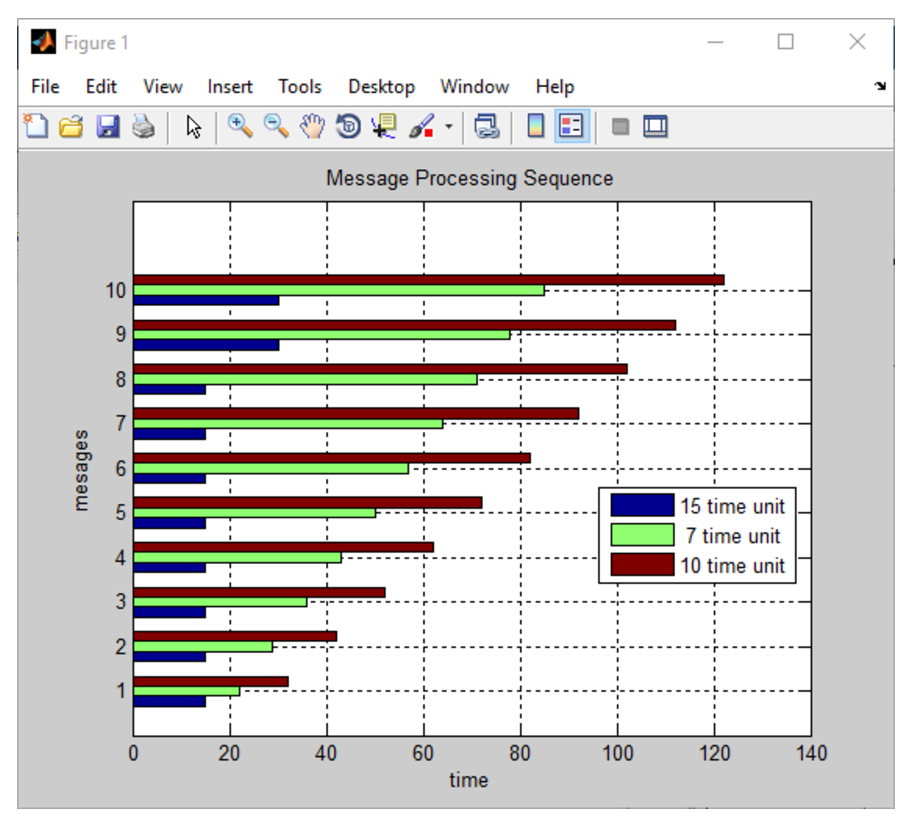
\includegraphics[width=1\linewidth]{./figs/graphic_sequence.eps}
 \caption{Sequence graph example.}
\label{fig:graphic_sequence}
\end{figure}
%
\begin{figure}[h]
\begin{minipage}[c]{0.49\linewidth}
\centering
 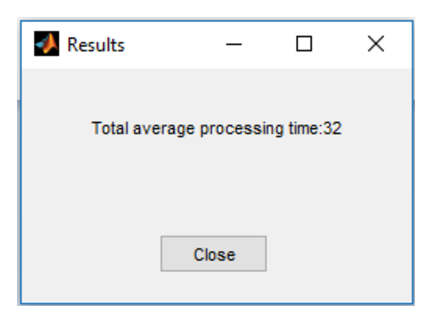
\includegraphics[width=0.8\linewidth]{./figs/outputs_FIFO.eps}
\end{minipage}
\begin{minipage}[c]{0.49\linewidth}
\centering
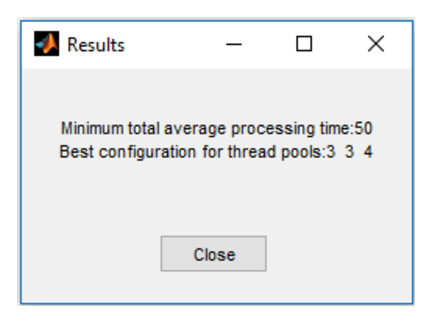
\includegraphics[width=0.8\linewidth]{./figs/outputs_PSO.eps}
\end{minipage}
\caption{Program output interface..}
\label{fig:outputs}
\end{figure}
%==============================================================================
\subsection{Scenarios}
\label{subsec:scenarios}
%==============================================================================
Para testar os programas criados para simulação preliminar do processamento das mensagens no fluxo de um processo de integração, utilizamos um cenário simplificado. Conforme a Figura~\ref{fig:workflow}, o fluxo de tarefas possui três tarefas, cujos tempos de processamento são respectivamente: 15, 7 e 10 unidades de tempo.
\begin{figure}[h]
\centering
 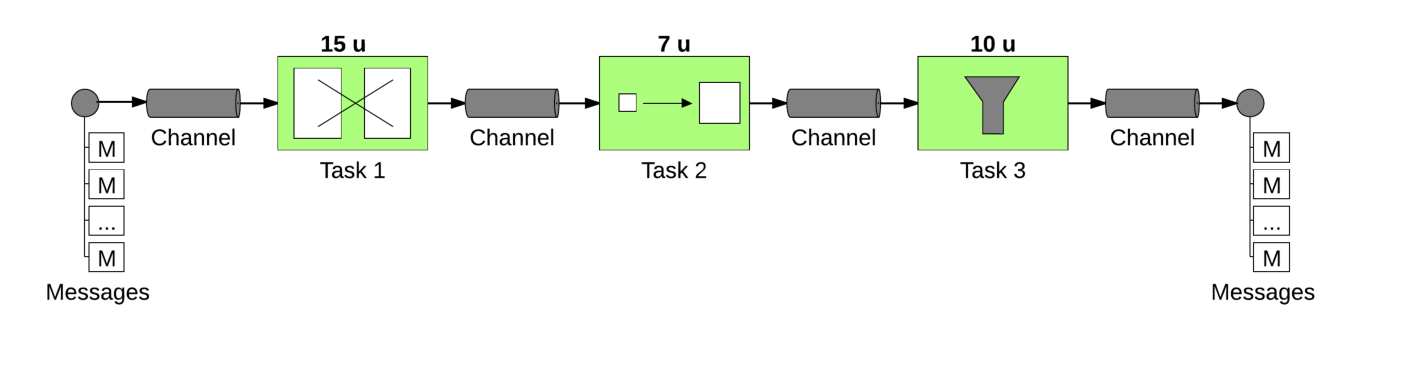
\includegraphics[width=1\linewidth]{./figs/workflow.eps}
 \caption{Workflow sample.}
\label{fig:workflow}
\end{figure}

Criamos vinte quatro cenários diferentes, variando o número total de mensagens a serem processadas: 10, 100, 1000, 10000 mensagens, sendo processadas por pools contendo 3, 4, 5, 6, 7, 8, 9 e 10 threads.
Os parâmetros de entrada utilizados foram:
\begin{itemize}
\item Número total de threads: de 3 a 10.
\item Número total de mensagens a serem processadas: 10, 100, 1000, 10000.
\item Número total de soluções testadas: 100
\item Vetor contendo os tempos de processamentos das tarefas: [15;7;10] 
\end{itemize}
%==============================================================================
\subsection{Actual system}
\label{subsec:actual_system}
%==============================================================================
% - trata-se da execução do "sistema atual" para coletar os valores para as variáveis selecionadas em cada cenário de experimentação
No modelo de agendamento das tarefas com um único pool de threads, todas as threads do pool se encarregam de executar a primeira tarefa, processando toda a carga inicial de mensagens que chega ao canal de entrada da primeira tarefa. Apenas, quando todas as mensagens terminam seu processamento por uma tarefa é que começam a ser processadas pela execução da tarefa subsequente. 

A figura~\ref{fig:graphic_sequence_single} mostra o processamento de mensagens do primeiro cenário, onde a carga inicial é de 10 mensagens, o pool contém 10 threads e o fluxo de processo de integração possui 3 tarefas, cujos tempos de processamento são respectivamente 15, 7 e 10 unidades de tempo. O pool de threads finaliza o processamento das mensagens pela primeira tarefa em 15 unidades de tempo, já que há 10 threads e 10 mensagens para serem processadas. De modo similar, finaliza o processamento das mensagens pela segunda tarefa em 7 unidades de tempos e pela terceira em 10 unidades de tempo. Nesse cenário, o tempo final de processamento de cada uma das mensagens é o mesmo: 32 unidades de tempo. Calculando a média aritmética desses tempos, acha-se que o tempo total médio de processamento das 10 mensagens é de 32 unidades de tempo.

\begin{figure}[h]
\centering
 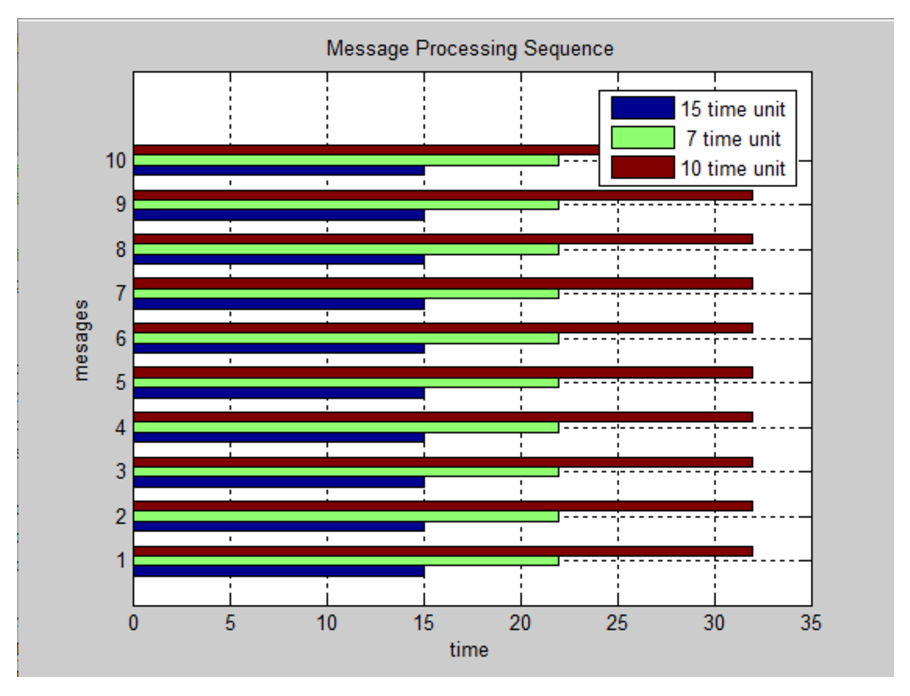
\includegraphics[width=1\linewidth]{./figs/graphic_sequence_single.eps}
 \caption{Processing sequence with single pool.}
\label{fig:graphic_sequence_single}
\end{figure}
%
%==============================================================================
% \subsubsection{Results}
% \label{subsubsec:results_actual_system}
%==============================================================================
%                  - apresentar gráficos/tabelas e, textualmente, descrever os resultados obtidos. Não se deve concluir nada nesta parte
A Figura~\ref{fig:fluxogram_FIFO} retrata o fluxograma do programa desenvolvido para simular esse processamento com cenários com uma carga de entrada com uma maior quantidade de mensagens. A Tabela~\ref{tab:TTAP_single} mostra os valores do tempo total médio de processamento obtidos com cada um dos cenários.
\begin{figure}[h]
\centering
 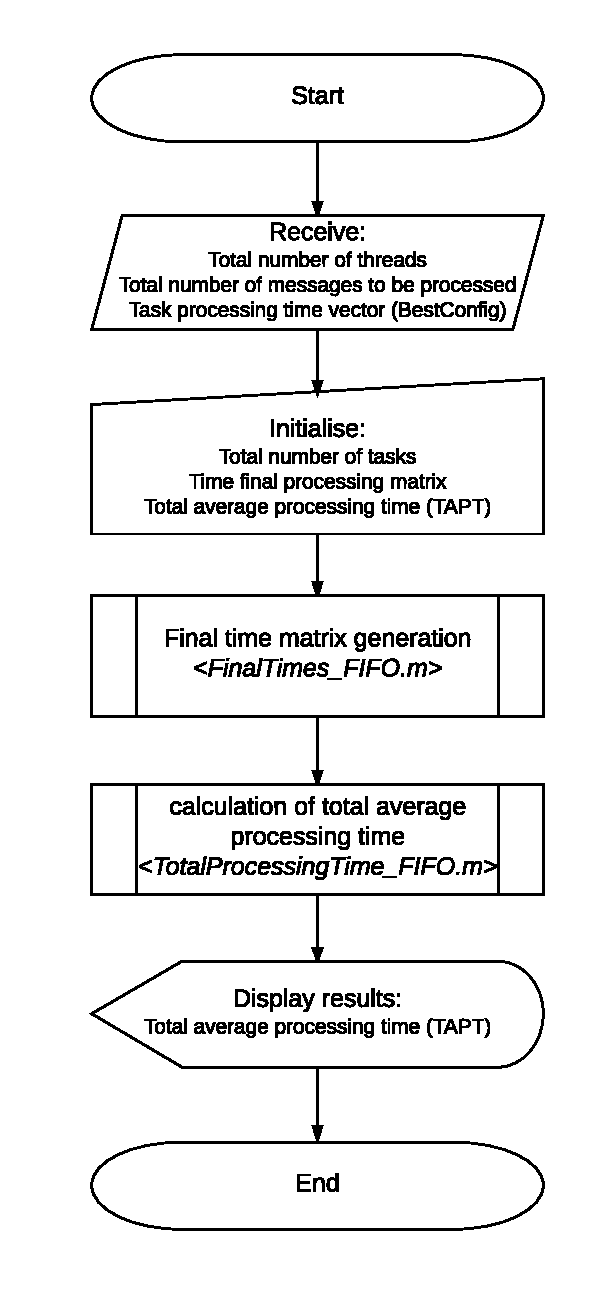
\includegraphics[width=0.7\linewidth]{./figs/fluxogram_FIFO.eps}
 \caption{Scheduling with single thread pool.}
\label{fig:fluxogram_FIFO}
\end{figure}
%
\begin{table}[htb]
\centering
\caption{TTAP with single pool.}
\label{tab:TTAP_single}
\begin{tabular}{cllll}
\hline
\multicolumn{1}{c}{Number of} & \multicolumn{4}{c}{Number of messages} \\
\multicolumn{1}{c}{threads}   & 10         & $10^2$      & $10^3$         & $10^4$    \\ \hline
3                             & 95.30      & 905.03      & 9005.00        & 90005.00        \\
4                             & 72.40      & 680.00      & 6755.00        & 67505.00        \\
5                             & 59.00      & 545.00      & 5405.00        & 54005.00        \\
6                             & 50.60      & 455.00      & 4505.00        & 45005.00        \\
7                             & 43.80      & 390.74      & 3862.14        & 38576.42        \\
8                             & 38.40      & 342.48      & 3380.00        & 33755.00        \\
9                             & 35.20      & 305.02      & 3005.00        & 30005.00        \\
10                            & 32.00      & 275.00      & 2705.00        & 27005.00        \\ \hline
\end{tabular}
\end{table}     

%==============================================================================
\subsection{Optimised system}
\label{subsec:optimised_system}
%==============================================================================
% - trata-se da execução do "sistema otimizado" para coletar os valores para as variáveis selecionadas em cada cenário de experimentação
No modelo de agendamento das tarefas com um múltiplos pools de threads, cada pool só executa a tarefa a qual está dedicado. Dessa forma, a carga inicial de mensagens que chega ao canal da primeira tarefa é processada no pool a ela destinado. Assim, quando uma mensagem termina de ser processada por uma tarefa, já pode ser processada na tarefa subsequente, desde que o haja threads disponíveis no pool dedicado a executar essa próxima tarefa. 

A figura~\ref{fig:graphic_sequence_multiple} mostra o processamento de mensagens no cenário: carga inicial com 10 mensagens; três pools contendo 8, 1, 1 threads, respectivamente; e um fluxo de processo de integração com três tarefas, cujos tempos de processamento são respectivamente 15, 7 e 10 unidades de tempo. Como o pool de threads dedicado a primeira tarefa possui 8 threads, ele finaliza o processamento de 8 mensagens em 15 unidades de tempo e as 2 restantes aguardam 15 unidades de tempo para que esse pool as execute, finalizando o processamento em 30 unidades de tempo. Como o segundo e o terceiro pool só possuem uma thread, O processamento será acrescido de 7 unidades de tempo a cada mensagem na segunda tarefa e em 10 unidades de tempo na terceira. 

\begin{figure}[h]
\centering
 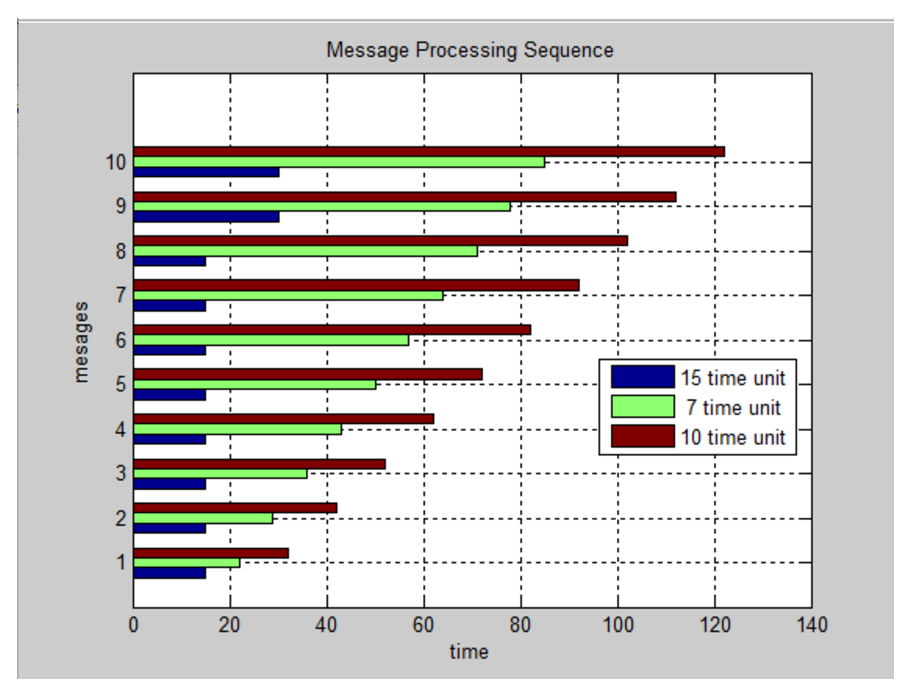
\includegraphics[width=1\linewidth]{./figs/graphic_sequence_multiple.eps}
 \caption{Processing sequence with multiple pools.}
\label{fig:graphic_sequence_multiple}
\end{figure}
%
A Tabela~\ref{tab:TFP} mostra os tempos finais de processamento (TFP) de cada uma das mensagem processadas. Calculando a média aritmética desses tempos, acha-se que o tempo total médio de processamento das 10 mensagens é de 77 unidades de tempo.
%
\begin{table}[htb]
\centering
\caption{TFP with multiple pools.}
\label{tab:TFP}
\begin{tabular}{cllll}
\hline
\multicolumn{1}{c}{Message} & \multicolumn{3}{c}{TFP in task} \\
							  & 1      & 2       & 3            \\ \hline
1                             & 15      & 22      & 32               \\
2                             & 15      & 29      & 42               \\
3                             & 15      & 36      & 52               \\
4                             & 15      & 43      & 62              \\
5                             & 15      & 50      & 72               \\
6                             & 15      & 57      & 82               \\
7                             & 15      & 64      & 92               \\
8                             & 15      & 71      & 102            \\
9                             & 30      & 78      & 112             \\
10                            & 30      & 85      & 122      \\ \hline
\end{tabular}
\end{table} 
% %==============================================================================
% \subsubsection{Results}
% \label{subsubsec:results_optimised_system}
%==============================================================================
%                  - apresentar gráficos/tabelas e, textualmente, descrever os resultados obtidos. Não se deve concluir nada nesta parte.
A Figura~\ref{fig:fluxogram} retrata o fluxograma do programa desenvolvido para simular esse processamento do modelo de múltiplo pools de threads em cenários com uma carga de entrada com uma maior quantidade de mensagens. A Tabela~\ref{tab:best_config} mostra os valores encontrados para as configurações do número de threads em cada pool, utilizando o algoritmo proposto, limitando o número de soluções a 100. A Tabela~\ref{tab:TTAP_multiplo} mostra os valores do tempo total médio de processamento obtidos com essas configurações em cada um dos cenários.
\begin{figure}[h]
\centering
 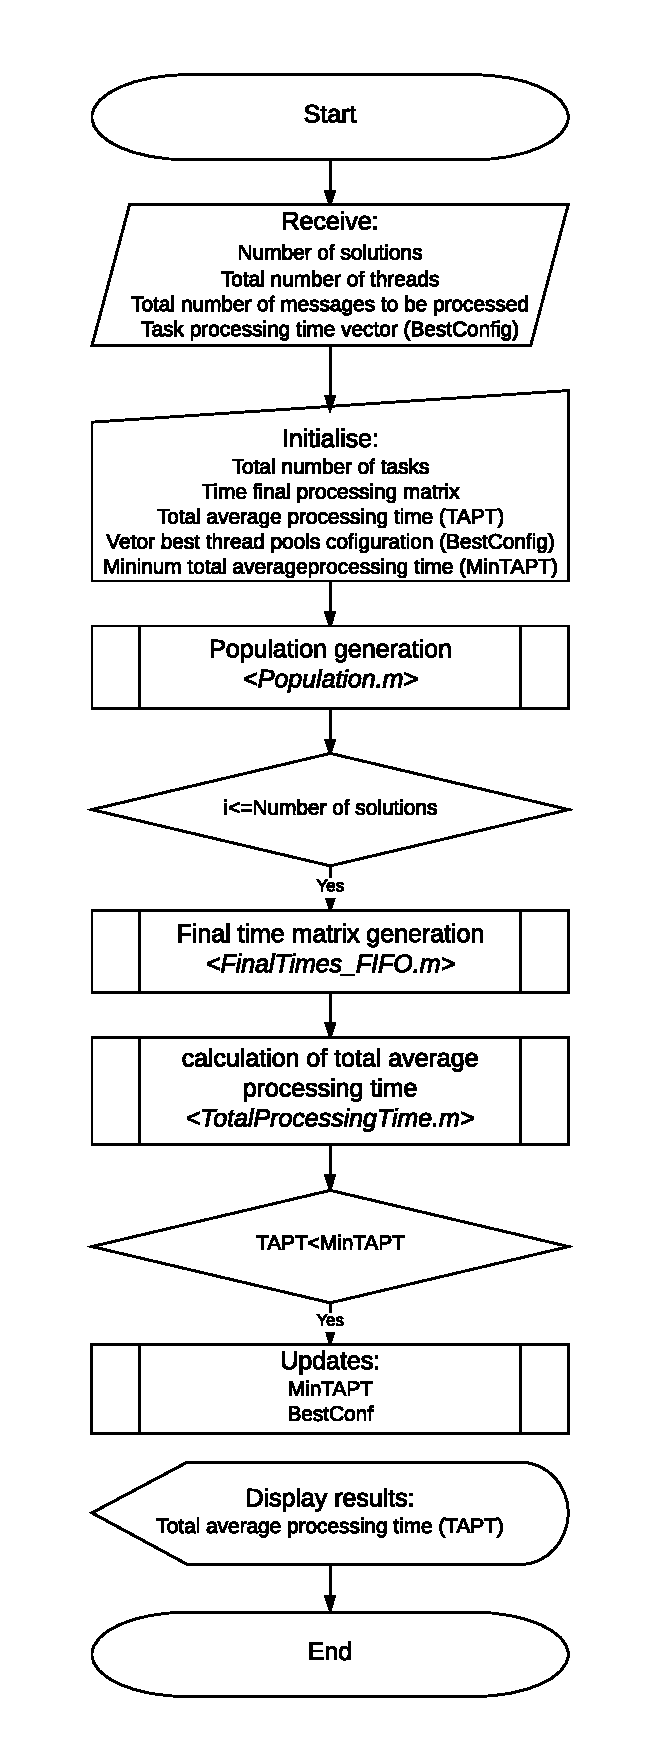
\includegraphics[width=0.8\linewidth]{./figs/fluxogram.eps}
 \caption{Scheduling with multiple pools.}
\label{fig:fluxogram}
\end{figure}
%
\begin{table}[htb]
\centering
\caption{Best configuration of the thread pools.}
\label{tab:best_config}
\begin{tabular}{cllll}
\hline
\multicolumn{1}{c}{Number of}  & \multicolumn{4}{c}{Number of messages} \\
\multicolumn{1}{c}{threads}   & 10           & $10^2$        & $10^3$         & $10^4$          \\ \hline
3                             & [1;1;1]      & [1;1;1]       & [1;1;1]        & [1;1;1]       \\
4                             & [2;1;1]      & [2;1;1]       & [2;1;1]        & [2;1;1]      \\
5                             & [2;1;2]      & [2;1;2]       & [2;1;2]        & [2;1;2]       \\
6                             & [2;2;2]      & [3;1;2]       & [3;1;2]        & [3;1;2]      \\
7                             & [3;2;2]      & [3;2;2]       & [3;2;2]        & [3;2;2]        \\
8                             & [4;2;2]      & [3;2;3]       & [3;2;3]        & [3;2;3]         \\
9                             & [4;2;3]      & [4;2;3]       & [4;2;3]        & [4;2;3]       \\
10                            & [4;2;4]      & [5;2;3]       & [5;2;3]        & [5;2;3]      \\ \hline
\end{tabular}
\end{table}  
%
\begin{table}[htb]
\centering
\caption{TTAP with multiple thread pools.}
\label{tab:TTAP_multiplo}
\begin{tabular}{cllll}
\hline
\multicolumn{1}{c}{Number of} & \multicolumn{4}{c}{Number of messages} \\
\multicolumn{1}{c}{threads}   & 10         & $10^2$       & $10^3$        & $10^4$          \\ \hline
3                             & 99.50      & 774.50       & 7524.50        & 75024.50       \\
4                             & 77.00      & 527.00       & 5027.00        & 50027.00       \\
5                             & 65.50      & 403.00       & 3778.00        & 37528.00       \\
6                             & 62.00      & 378.50       & 3528.50        & 35028.50       \\
7                             & 54.00      & 279.45       & 2529.49        & 25029.49        \\
8                             & 52.00      & 277.00       & 2526.83        & 25026.83        \\
9                             & 47.80      & 216.73       & 1904.24        & 18779.24        \\
10                            & 46.50      & 204.97       & 1779.99        & 175529.99        \\ \hline
\end{tabular}
\end{table}  
%==============================================================================
\subsection{Discussion}
\label{subsec:discussion}
%==============================================================================
%               - analisar os resultados obtidos, buscando explicar valores que possam chamar atenção em cada técnica e comparar os valores obtidos a partir do "optimised model" com aqueles obtidos no "actual system" para avaliar possíveis ganhos.
A Figura~\ref{fig:comparasion} apresenta quatro gráficos comparando o tempo total médio de processamento do modelo utilizando única thread e do modelo utilizado múltiplos pools com o número de threads de cada pool, encontrado pelo algoritmo de otimização. Cada gráfico corresponde a simulação do processamento de 10, 100, 1000 e 10000 mensagens, respectivamente, utilizando pools variando de 3 a 10 threads. 

\begin{figure}[htp]
\centering
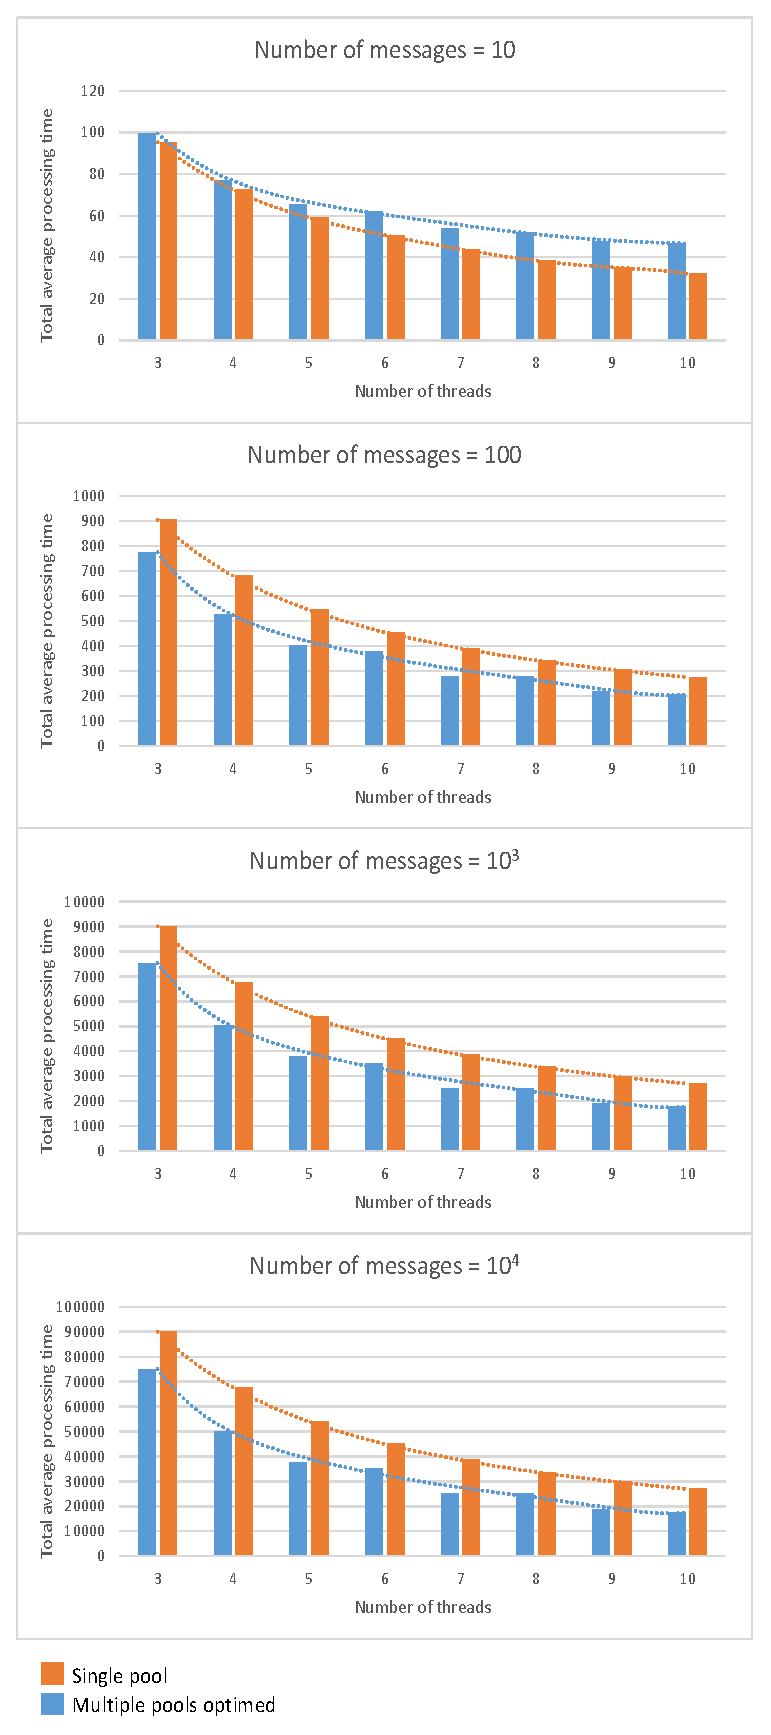
\includegraphics[width=1\linewidth]{./figs/comparasion.eps}
\caption{TTAP with single and multiple threads pools.}
\label{fig:comparasion}
\end{figure}

As barras indicam o valor do TTAP para cada quantidade de threads em ambos os modelos. No primeiro gráfico, com a simulação do processamento de uma carga inicial de 10 mensagens, percebemos que o modelo com o único pool de threads fornece menor TTAP do que o modelo com múltiplos pools e essa diferença aumenta, quando aumentamos o número de threads nos pools. Porém, nos demais gráficos, percebemos que o modelo com múltiplos pools, configurados com o número de threads ótimo, ou perto de ótimo, fornece menor TTAP do que o modelo com único pool. A Tabela~\ref{tab:TTAP_difference} mostra o valor absoluto da diferença entre o TTAP do modelo com único pool e o modelo múltiplos pools, sendo que os valores máximos em cada caso, estão destacados com o símbolo "*". Dos cenários testados, apenas com a carga inicial igual a 10 mensagens, o modelo com único pool foi melhor que o modelo com múltiplos pools de threads, nos demais cenários o modelo proposto apresentou melhores resultados. A diferença atingiu 17478 unidades de tempo a menos no TTAP, utilizando o modelo proposto, quando a carga inicial foi de 10000 mensagens. 
%
\begin{table}[htb]
\centering
\caption{Difference between TTAP.}
\label{tab:TTAP_difference}
\begin{tabular}{cllll}
\hline
\multicolumn{1}{c}{Number of} & \multicolumn{4}{c}{Number of messages} \\
\multicolumn{1}{c}{threads}   & 10         & $10^2$       & $10^3$        & $10^4$          \\ \hline
3                             & 4.20      & 130.53       & 1480.50        & 14980.50       \\
4                             & 4.60      & 153.00*       & 1728.00*        & 17478.00*       \\
5                             & 6.50      & 142.00       & 1627.00        & 16477.00      \\
6                             & 11.40      & 76.56       & 976.50          & 9976.50      \\
7                             & 10.20      & 111.29       & 1332.65        & 13546.93       \\
8                             & 13.60      & 65.48       & 853.17         & 8728.17       \\
9                             & 12.60      & 88.26       & 1100.76        & 11225.76        \\
10                            & 14.50*     & 70.03       & 925.01        & 9475.01        \\ \hline
\end{tabular}
\end{table}  

Os gráficos também apresentam a linha de tendência estatística do TTAP, representada por linhas pontilhadas. A análise por linhas de tendência, também chamada de análise de regressão, permite entender o comportamento de uma variável resposta, por meio de uma equação matemática e assim prever resultados futuros. Uma linha de tendência é mais precisa quanto maior o valor de R-quadrado. R-quadrado é o coeficiente de determinação, número que varia de 0 a 1 e que permite estimar o quanto podemos predizer a variável resposta (TTAP, no nosso caso), a partir da variável preditora (número de threads). Assim, as linhas de tendência apresentadas nos gráficos correspondem a uma equação polinomial, que explica o comportamento do TTAP em relação ao número de threads, permitindo prever o valor de TTAP para uma maior quantidade de threads nos pools. A Tabela~\ref{tab:tendency_line} apresenta essas equações e o R-quadrado correspondente.
%
\begin{table*}[htb]
\centering
\caption{Statistical trend of the TTAP.}
\label{tab:tendency_line}
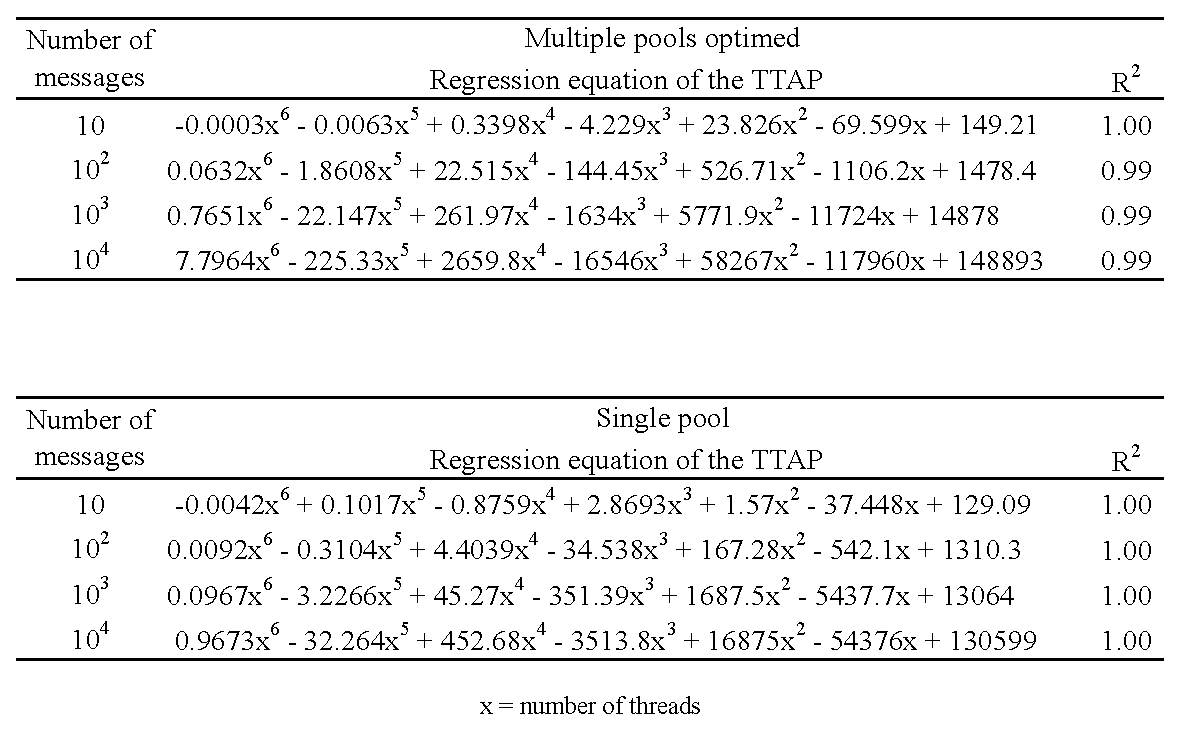
\includegraphics[width=0.7\linewidth]{./figs/equation.eps}
\end{table*}  
%
Assim, as simulações nos cenários apresentados dão indícios de que, a medida que a carga de entrada das mensagens cresce, aumenta a vantagem de se utilizar o modelo com múltiplos pools de threads.

